\chapter{Controls}
\label{ch:controls}
Control systems are responsible for computing the commands necessary for actuators to cause the trajectory of a system to go from its current state to a desired state. There are many different methods that can be used to determine the output commands. One of the more popular and widely implemented control systems is the PID (Proportional, Integral, Differential) controller. Lyapunov controllers utilize knowledge of the system dynamics to compute appropriate output commands. The robots in these experiments originally used PID controllers for position and heading control and were later tested with a Lyapunov contoller.

\section{PID}
\label{sec:pid}
PID controllers use the current state estimate to determine the errors between the desired state and the current state. The goal of the PID controller is to drive those errors to zero based on a number of criterion including rise time, settling time, steady state error and overshoot (see Figure \ref{fig:pid}).

\begin{figure}[ht!]
	\centering
	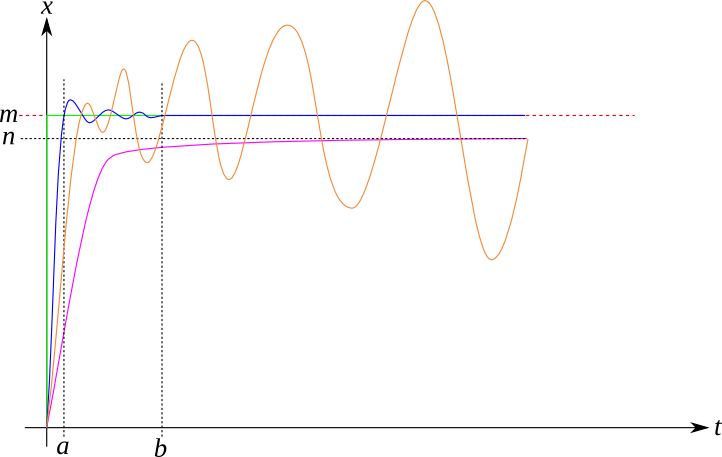
\includegraphics[width=.75\textwidth]{images/pid}
	\caption{PID controller output. The green line is the ideal output while the blue and purple lines are typical results. The orange line shows what happens when a system becomes unstable. Point $m$ represents the desired state, $m-n$ represents steady state error, point $a$ is the rise time and point $b$ is the settling time.}
	\label{fig:pid}
\end{figure}

There are separate PID controllers used for each of $x$ position, $y$ position and robot heading ($\psi$). The process used to compute an output using a PID controller uses three separate errors and a gain for each of those errors. Looking at the PID controller for heading the errors are

\begin{align}
\label{eq:piderrors}
\begin{split}
E_P &= \psi_{\text{ref}_k} - \psi_k \\
E_I &= \sum_{i=0}^{k}E_{P_i}*\Delta T \\
E_D &= \frac{\psi_k - \psi_{k-1}}{\Delta T}
\end{split}
\end{align}
where $\psi_{\text{ref}_k}$ is the desired heading at the current time, $\psi_k$ is the current heading estimate, $\psi_{k-1}$ is the previous heading estimate and $\Delta T$ is the time elapsed since the last PID control calculation was performed. The contribution of each error is then weighted by a gain to obtain the final output command, $u$, such that

\begin{align}
\label{eq:pidcommand}
u = K_P*E_P + K_I*E_I + K_D*E_D
\end{align}
where $K_P$ is the proportional gain, $K_I$ is the integral gain and $K_D$ is the differential gain.

The only parameters available to tune PID controllers for performance are the gains. There are some rules of thumb for tuning gains properly as described in \cite{ZeiglerNichols42} that can work as a good starting point. The difficulty in using PID controllers for the small robots used in these experiments is that the gains must be tuned for specific operating scenarios so that a set of gains that work well at full speed on asphalt do not work at all when the robot is driving in soft sand at any velocity. PID controllers work best when they only have to reject a small range of disturbances and the small robots are required to be operated in environments with a large range of disturbances.

When the characteristics of a robot are changed the PID gains must also be modified to reflect those changes. These characteristics include mass, center of mass, particular treads or motors and payloads, as these all affect the dynamics of the system. Gain scheduling is the process of tuning a system to use a different set of gains based on the operating environment or characteristics of the robot, however this is very time consuming. This motivates the search for a better control system for these small robots.

\section{Lyapunov}
\label{sec:lyapunov}
*** Talk about how Lyapunov controllers work \cite{Khalil02}. ***

\subsection{Unicycle-like Robot Kinematics}
\label{sec:unicycleKinematics}
\cite{Rusu05RobotuxLyapunov,Aicardi_UnicycleLyapunov95} describes a method for using a Lyapunov controller for a differential drive robot, similar in nature to the small robots considered in these experiments. This class of robot is typically referred to as a unicycle-like robot in the literature. This section will mostly be a restatement of their work but with more intermediate steps and a slightly different formulation included to make the derivation easier to follow and to show how some of the code changes in Appendix \ref{sec:lyapunovcode} were motivated and justified when extending the work of \cite{Rusu05RobotuxLyapunov}.

\begin{figure}[ht!]
	\centering
	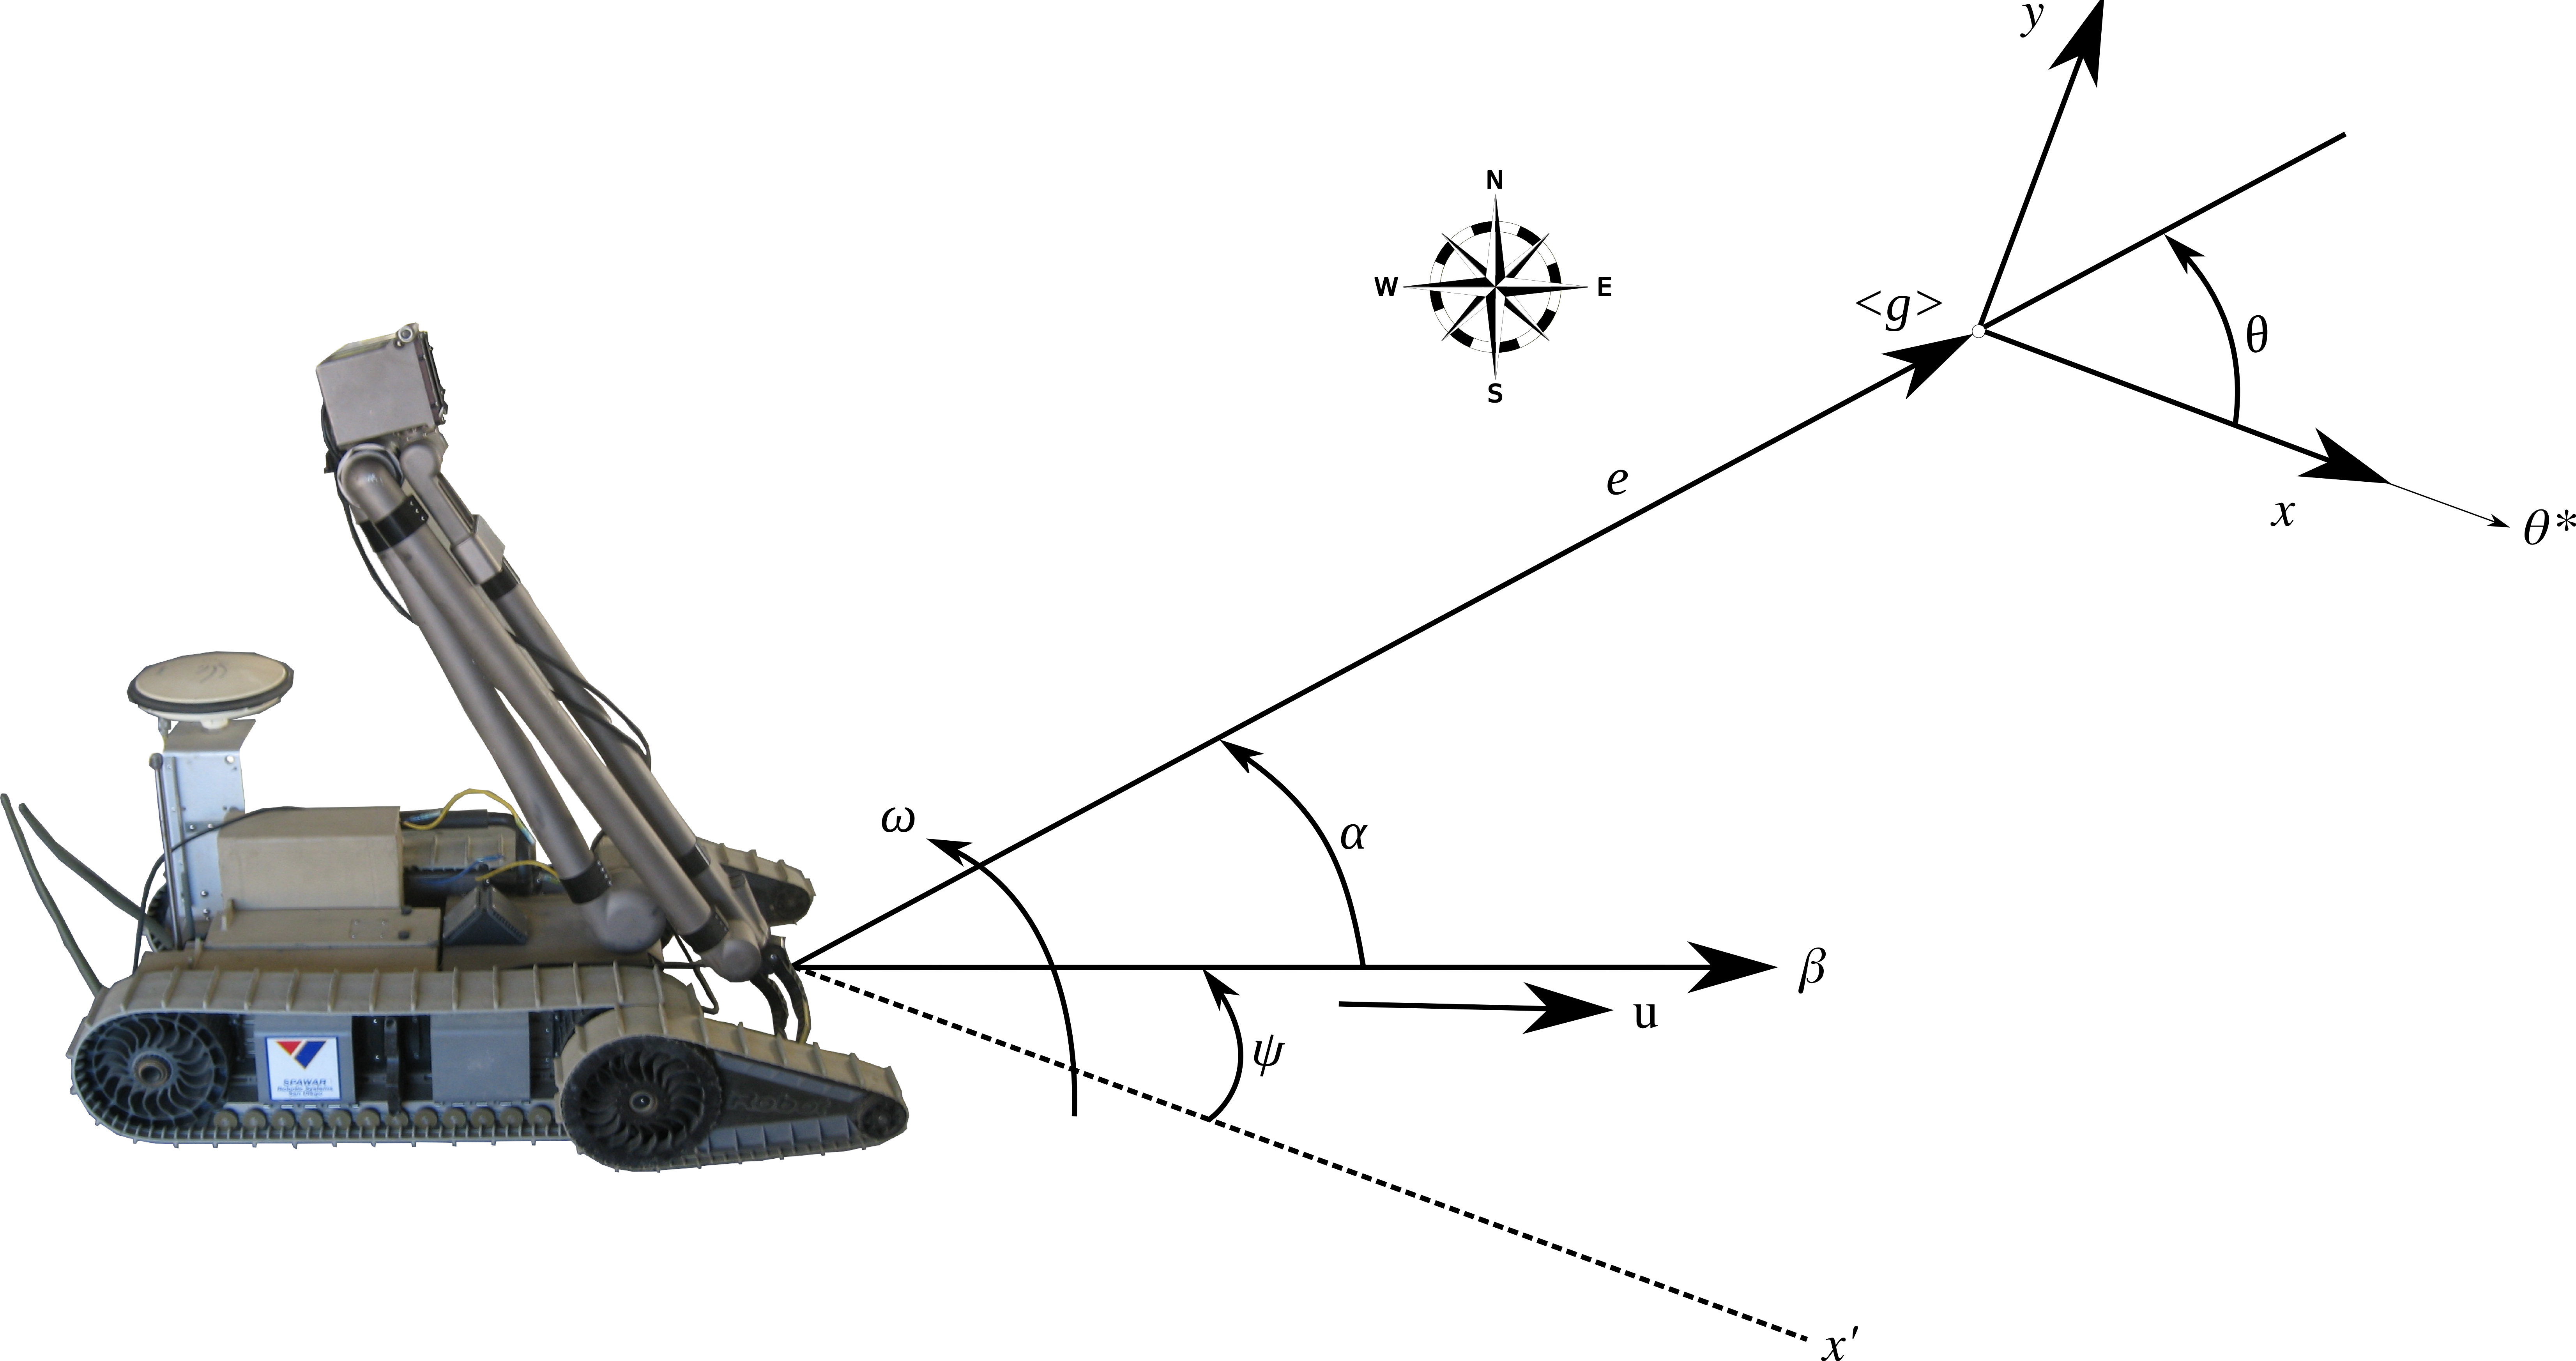
\includegraphics[width=.95\textwidth]{images/packbotlyapunov}
	\caption{PackBot with coordinates for the Lyapunov controller.}
	\label{fig:pblyapunov}
\end{figure}

Figure \ref{fig:pblyapunov} will be used as the basis for the equations that follow and will be explained in further detail here. Given a robot at some initial position we want it to move to a goal position with a specific heading where the goal position is the origin of the $<g>$ coordinate system and the desired heading is along the $x$-axis. The states that define the robot's current position, heading, and linear and angular velocities are being calculated using the Kalman filter of \S\ref{sec:extendedkf} whereas the goal position and heading are given as inputs to the robot. Note that the linear velocity is given by $u$ and the angular velocity by $\omega$. The control system attempts to force three separate errors to zero:
\begin{itemize}
\item the translational error $e$,
\item the angle determined using an extension of the vector $e$ into $<g>$ and represented by $\theta$,
\item the error between $\theta$ and the current heading shifted to the $<g>$ coordinate system, $\psi$, where the error is given by $\alpha$.
\end{itemize}

Since unicycle-like robots exhibit non-holonomic constraints (they are only able to move forwards or backwards along the direction of their current heading and are not able to perform strafing maneuvers) it is necessary to use all three errors in the control system. The errors can all be calculated using the inputs to the robot of a goal position and heading and the state estimates of the Kalman filter.

A kinematic model of the robot is used to predict how the robot moves

\begin{align}
\label{eq:lyapunovkinematics1}
\begin{split}
\dot{x} &= u\cos(\psi) \\
\dot{y} &= u\sin(\psi) \\
\dot{\psi} &= \omega.
\end{split}.
\end{align}
The expressions in (\ref{eq:lyapunovkinematics1}) are then converted to a polar coordinate representation via a coordinate transformation and give expressions for the errors that the control system is attempting to drive to zero with the errors as shown in Figure \ref{fig:pblyapunov}

\begin{align}
\label{eq:lyapunovkinematics2}
\begin{split}
e &= \sqrt{x^2+y^2} \\
\theta &= \atanh(y,x) \\
\alpha &= \theta - \psi.
\end{split}
\end{align}
Combining (\ref{eq:lyapunovkinematics2}) with (\ref{eq:lyapunovkinematics1}) results in

\begin{align}
\label{eq:lyapunovkinematics3}
\begin{split}
\dot{e} &= -u*\cos(\theta-\psi) \\
\dot{\theta} &= u\frac{\sin\alpha}{e} \\
\dot{\psi} &= \omega.
\end{split}
\end{align}
Finally, replacing $\alpha$ with $\theta-\psi$ results in a kinematic model of

\begin{align}
\label{eq:lyapunovkinematics}
\begin{split}
\dot{e} &= -u\cos\alpha \\
\dot{\alpha} &= -\omega + u\frac{\sin\alpha}{e} \\
\dot{\theta} &= u\frac{\sin\alpha}{e}.
\end{split}
\end{align}

\subsection{Control Lyapunov Function}
\label{sec:controllyapunov}
The control Lyapunov function is selected to be positive and contain all three error states and is given by

\begin{align}
\label{eq:lyapunovfunction}
V = V_1 + V_2 = \frac{1}{2}\lambda e^2 + \frac{1}{2}\left(\alpha^2+h\theta^2\right)
\end{align}
where $\lambda$ and $h$ are positive constants that can be used to tune the controller output (see \S\ref{sec:trajectoryCurvature}). Using the kinematics equations in (\ref{eq:lyapunovkinematics}) the derivative of each term of the candidate control Lyapunov function can be found as

\begin{align}
\label{eq:Vderivatives}
\begin{split}
\dot{V}_1 &= \lambda e\dot{e} = \lambda e (-u\cos\alpha) = -\lambda eu\cos\alpha \\
\dot{V}_2 &= \alpha\dot{\alpha}+h\theta\dot{\theta} \\
&= -\alpha\omega + \alpha u\frac{\sin\alpha}{e} + h\theta u\frac{\sin\alpha}{e} \\
&= \alpha\left(-\omega + u\frac{\sin\alpha}{e} + h\theta u\frac{1}{\alpha}\frac{\sin\alpha}{e}\right) \\
&= \alpha\left(-\omega + u\frac{\sin\alpha}{\alpha}\frac{(\alpha+h\theta)}{e}\right)
\end{split}
\end{align}
and from there the total derivative is found as

\begin{align}
\label{eq:lyapunovfunctionderivative}
\begin{split}
\dot{V} &= \dot{V}_1 + \dot{V}_2 = -\lambda e u\cos\alpha + \alpha\left(-\omega+u\frac{\sin\alpha}{\alpha}\frac{(\alpha+h\theta)}{e}\right).
\end{split}
\end{align}

Now it needs to be shown that $\dot{V}\leq0$ which can be done by showing that $\dot{V}_1\leq0$ and $\dot{V}_2\leq0$. This is true for $\dot{V}_1$ if $u$ takes the form

\begin{align}
\label{eq:lyapunovu}
u = \gamma e\cos\alpha
\end{align}
where $\gamma$ is a positive constant different from $\lambda$. Substituting this value of $u$ into (\ref{eq:Vderivatives}) results in

\begin{align}
\label{eq:V1dotfinal}
\dot{V}_1 = -\lambda eu\cos\alpha = -\lambda\gamma e^2\cos^2\alpha.
\end{align}
Since $V_1\geq0$ and $\dot{V}_1\leq0$ we have that $V_1$ converges asymptotically to a positive defined limit.

Replacing $u$ in the expression for $\dot{V}_2$ in (\ref{eq:Vderivatives}) results in

\begin{align}
\label{eq:V2dotreplaceu}
\begin{split}
\dot{V}_2 &= \alpha\left(-\omega+u\frac{\sin\alpha}{\alpha}\frac{(\alpha+h\theta)}{e}\right) \\
&= \alpha\left(-\omega+\gamma e\frac{\cos\alpha\sin\alpha}{\alpha}\frac{(\alpha+h\theta)}{e}\right) \\
&= \alpha\left(-\omega+\gamma(\alpha+h\theta)\frac{\cos\alpha\sin\alpha}{\alpha}\right).
\end{split}
\end{align}
Similarly, $\dot{V}_2$ is negative if $\omega$ takes the form

\begin{align}
\label{eq:lyapunovomega}
\begin{split}
\omega &= k\alpha + \gamma\frac{\cos\alpha\sin\alpha}{\alpha}\left(\alpha+h\theta\right)
\end{split}
\end{align}
where $k$ is a positive constant. Substituting this value of $\omega$ into (\ref{eq:V2dotreplaceu}) gives

\begin{align}
\label{eq:V2dotfinal}
\begin{split}
\dot{V}_2 &= \alpha\left(-k\alpha-\gamma\frac{\cos\alpha\sin\alpha}{\alpha}(\alpha+h\theta) + \gamma\frac{\cos\alpha\sin\alpha}{\alpha}(\alpha+h\theta)\right) \\
&= -k\alpha^2 \leq 0.
\end{split}
\end{align}
and $V_2$ converges asymptotically to a positive defined limit.

Substituting $\dot{V}_1$ from (\ref{eq:V1dotfinal}) and $\dot{V}_2$ from (\ref{eq:V2dotfinal}) into the expression for $\dot{V}$ yields

\begin{align}
\label{eq:Vfinal}
\dot{V} = \dot{V}_1 + \dot{V}_2 = -\lambda\gamma e^2\cos^2\alpha - k\alpha^2 \leq 0.
\end{align}
This expression is equal to zero only when $\alpha=0$ \textit{and} $e=0$, which only occurs when the robot has reached its goal pose. Therefore, at any point along the robots trajectory other than the goal point this function is negative definite and is asymptotically stable.

Using the expressions for $u$ in (\ref{eq:lyapunovu}) and $\omega$ in (\ref{eq:lyapunovomega}) and substituting those values back into the kinematic model from (\ref{eq:lyapunovkinematics}) gives

\begin{align}
\label{eq:lyapunovfinalkinematics}
\begin{split}
\dot{e} &= -\gamma e\cos^2\alpha \\
\dot{\alpha} &= -\left(k\alpha + \gamma h\frac{\cos\alpha\sin\alpha}{\alpha}\right) \\
\dot{\theta} &= \gamma\cos\alpha\sin\alpha
\end{split}
\end{align}

Combining (\ref{eq:lyapunovu}) and (\ref{eq:lyapunovomega}) gives the control law to replace the PID controller from \S\ref{sec:pid}:

\begin{align}
\label{eq:lyapunovControlLaw}
\begin{split}
u &= \gamma e\cos\alpha \\
\omega &= k\alpha + \gamma\frac{\cos\alpha\sin\alpha}{\alpha}\left(\alpha+h\theta\right)
\end{split}
\end{align}

\subsection{Curvature of Resulting Trajectory}
\label{sec:trajectoryCurvature}
*** Say something about how the parameters $h$, $k$ and $\gamma$ in (\ref{eq:lyapunovControlLaw}) determine the curvature of the resulting trajectory. The important thing to recognize is that, even though there are three parameters to tune with the control Lyapunov function, a stable trajectory is guaranteed with control Lyapunov functions and the parameters affect only the curvature of the trajectory. With PID controllers there are more parameters to tune and they affect whether the resulting control law is stable as well as the response profile. The free parameters for Lyapunov are considered design variables and are beneficial. ***